\section*{Teoría}

\begin{enumerate}
    \item ¿Para qué es y en qué casos se usa el usuario \texttt{root}? ¿En qué casos no se usa o no debe usarse?
    
    Para Linux y macOS, el usuario root es el superusuario. Esto significa que tiene el mayor nivel de privilegios para 
    realizar cualquier acción en el sistema, modificar cualquier archivo, instalar software, cambiar la configuración 
    del sistema y ejecutar cualquier comando, sin restricciones.

    Si bien suena increible tener todo el control en el sistema hay desventajas, por ejemplo entornos compartidos, 
    para servidores o sistemas compartidos, es recomendable limitar el uso del usuario root a tareas estrictamente 
    necesarias y utilizar cuentas con privilegios más restringidos para las tareas diarias. \cite*{UserRoot}

    
    \item ¿Cuál es la diferencia entre \texttt{su} y \texttt{sudo}? \cite*{RootSU}
    
    \begin{itemize}
        \item \texttt{su}: Al ejecutar \texttt{su}, se cambia de usuario y convertirte en 
        el superusuario (root), que tiene permiso para hacer cualquier cosa en el sistema.

        \item \texttt{sudo}: Lo mismo que arriba pero es temporal, permite ejecutar el comando como 
        super usuario y recordará la contraseña como por 15 min, despues la volverá a pedir.
    \end{itemize}
    
    \item ¿Para qué sirve \texttt{chmod}? ¿Cómo se usa?
    
    El programa de línea de comandos chmod, abreviatura de change mode (cambiar modo en inglés), 
    chmod sirve para asignar permisos de acceso a carpetas y directorios en sistemas de archivos 
    compatibles con los permisos de archivo típicos de Unix.\\

    En Unix, el sistema de permisos de acceso a los archivos se basa en dos elementos fundamentales: 
    las clases de usuario y los permisos básicos individuales. En la gestión de estos permisos, 
    chmod soporta dos modos diferentes: la notación simbólica con letras (modo simbólico o carácter) 
    y la atribución de permisos con códigos octales de cifras (modo octal).


    ¿Cómo se usa? \texttt{chmod [opciones] modo archivo}


    \begin{itemize}
        \item opciones: Son parámetros adicionales que modifican el comportamiento del comando.
        \item modo: Especifica los nuevos permisos. Puede ser en formato numérico u octal (más común) o simbólico.
        \item archivo: El archivo o directorio al que se aplicarán los cambios.
    \end{itemize}
    
    Por ejemplo:
    \begin{center}
        chmod 755 archivo.txt    
    \end{center}

    Asigna permisos de lectura, escritura y ejecución al propietario, lectura y ejecución al grupo, y 
    lectura y ejecución a otros.


    \item Genera un pequeño pipeline de los comandos vistos durante la práctica, por ejemplo:
    \begin{enumerate}
        \item Crear una carpeta con un nombre.
        \item Crear un archivo.
        \item Con \texttt{traceroute}, generar una búsqueda y guardar el resultado en dicho archivo.
        \item Visualizar el contenido con \texttt{cat}, \texttt{head}, o \texttt{less} de dicho archivo.
        \item Modificar los permisos de lectura y escritura de este.
    \end{enumerate}
    
\begin{verbatim}
    # 1. Crear una carpeta 
    mkdir practica01
    
    # 2. Crear un archivo dentro de la carpeta
    touch practica01/ejercicoTeoria.txt
    
    # 3. Con traceroute, generar una búsqueda y guardar el resultado en dicho archivo
    traceroute www.google.com > practica01/ejercicoTeoria.txt
    
    # 4. Visualizar el contenido con cat
    cat practica01/ejercicoTeoria.txt    
    
    # 5. Modificar los permisos de lectura y escritura
    chmod 644 practica01/ejercicoTeoria.txt

    # 6. Ver los permisos 
    ls -l practica01/ejercicoTeoria.txt
\end{verbatim}

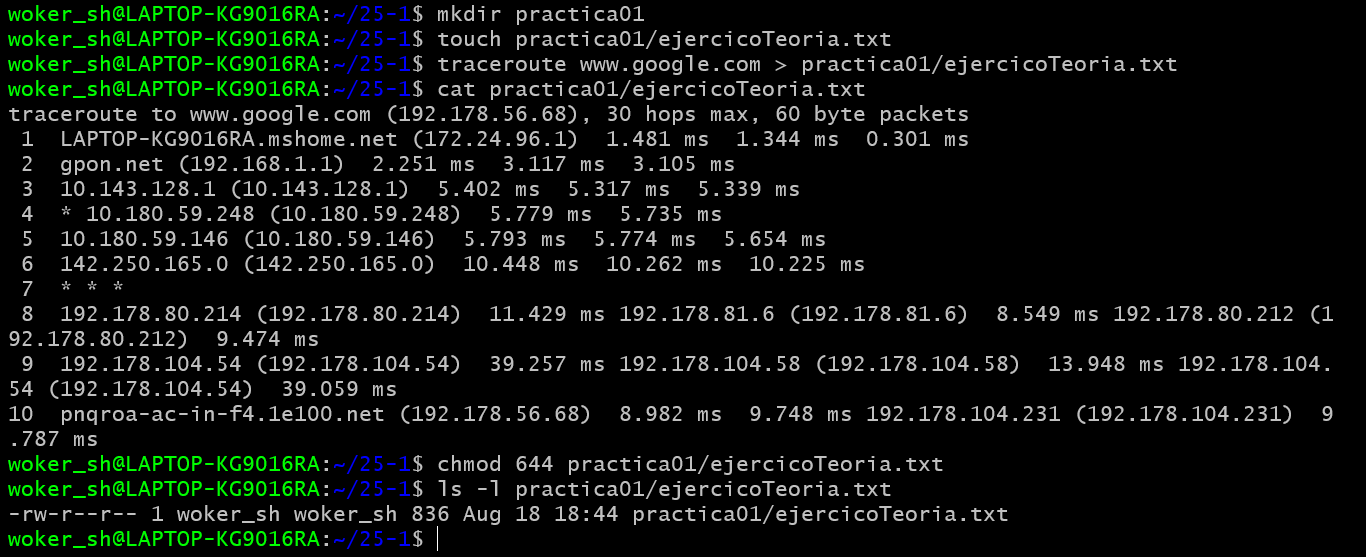
\includegraphics[scale = .3]{IMAGE/Ejercicio2/T05.png}

    \item Por último, añade lo aprendido de esta práctica, así como las posibles complicaciones que tuviste al realizarla.
\end{enumerate}
\begin{center}

    \item Carlos Daniel Cortés Jiménez: Me pareción intereante la practica ya que hubo muchos comandos que no conocía, y a su vez se me complicó al principio ejecutarlos ya que no escribía como debe de usarse algunos comandos. Después de ver guías y leer en internet me resultó más fácíl de lo que pense, también he de decir que lo que mas se me dificultó entender y aún tengo dudas son todos los apartados que da como resultado el realizar ifconfig.
    
    \item Marco Silva Huerta: A pesar de ya tener conocimientos previos de semestres anteriores sobre algunos comandos vistos en la practica, me resultó muy interesante. Pude refrescar y recordar el uso de comandos conocidos y a su vez aprender nuevas opciones y banderas me que a mi parecer resultó útil ver como combinar varias banderas para optimizar el uso de comandos, algo que no solía hacer con frecuencia. En general, fue una practica muy divertida que me facilitó recordar y aplicar comandos de manera más eficiente.
    
    \item Giovanny Cruz: Aprendi el uso de muchos comandos que no conocia. Al principio me costo un poco entender el uso de las banderas,
            pero despues de un rato de practica, se me hizo mas facil. Cre que lo que mas me costo, fue un poco el entender como usar varias 
            banderas al mismo tiempo, pero es muy util para hacer mas eficiente el uso de los comandos.

    \item Jonathan Martínez: La mayoría de los comandos que tuvimos que investigar no los conocía, quizá algunos los había usado con 
            anterioridad pero no consciente de su funcionamiento total. Revisar el manual de los comandos ayudó mucho a comprender su 
            funcionamiento.

    \item Edgar Montiel Ledesma: Volvo a recordar muchas vanderas utilies en esta practica ya que si los conocia pero, no es frecuente el uso de estos en el dia a dia, es bueno tener esta tarea para tenerlos presentes y hacer mas facil las actividades, por otro lado gracias al comando de man es mas facil poder recordarlos en el momente que se necesiten.
    
\end{center}
